\chapter{Modal EM for GSPNs}
\label{cap:algorithm}

The direct application of Modal EM, as discussed in Chapter \ref{cap:gmm}, to SPNs is intractable due to the large number of components in the mixture, which corresponds to the number of induced trees in the SPN. To address this limitation, we devised an adaptation of Modal EM that leverages the recursive nature of SPNs.

Our contribution has been published in a conference \citep{Madeira2022}, but we have revised the notation to present it with more clarity in this chapter. Additionally, we will provide a proof of the ascending property of the algorithm (Theorem \ref{thm:alg_correctness}) which was not included in the paper.

In this chapter, we will first introduce Modal EM for GSPNs algorithm and show how it was constructed (Section \ref{sec:algorithm:intro}), then we will prove its correctness (Section \ref{sec:algorithm:proof}). Next, we will discuss two applications: MAP inference and clustering (Section \ref{sec:algorithm:applications}).

\section{The algorithm}
\label{sec:algorithm:intro}

\textbf{Modal EM for GSPNs} traverses the network from bottom to top, and each node propagates $2n$ values. Each iteration of it takes $\Theta\left(n|\mathcal{S}|\right)$, where $n$ is the number of RVs, and $|\mathcal{S}|$ is the number of nodes in the GSPN. The pseudo-code is presented in Algorithm \ref{alg:mem}.

\begin{algorithm}[h]
  \caption{Modal EM for GSPNs}
  \label{alg:mem}
  \begin{algorithmic}
    \Input{a GSPN $\mathcal{S}$ over $X_1, \cdots, X_d$ and a point $\mathbf{x}^{(r)} \in \mathbb{R}^d$}
    \Output{a point $\mathbf{x}^{(r+1)} \in \mathbb{R}^d$ such that $\mathcal{S}\left(\mathbf{x}^{(r+1)}\right) \geq \mathcal{S}\left(\mathbf{x}^{(r)}\right)$}
  \end{algorithmic}
  \begin{algorithmic}[1]
    \ForAll{node $u$ of $\mathcal{S}$ in reverse topological order}
    \If{$u$ is a leaf}
    \LineComment{Let $X_i$ be the RV in the scope of $u$;}
    \LineComment{Let $\mu$ and $\sigma$ be the parameters of the Gaussian of $u$.}
    \State $N^u_i \gets \frac{u\left(x^{(r)}_i\right)\mu}{\sigma^2}$,  $D^u_i \gets \frac{u\left(x^{(r)}_i\right)}{\sigma^2}$ \label{alg:mem:leaf:1}
    \ForAll{RV $X_j \neq X_i$}
    \State $N^u_j \gets D^u_j \gets u\left(x^{(r)}_i\right)$ \label{alg:mem:leaf:2}
    \EndFor
    \ElsIf{$u$ is a product node}
    \ForAll{RV $X_i$} \label{alg:mem:product}
    \State $N^u_i \gets \prod_{v \in \ch(u)} N^v_i$
    \State $D^u_i \gets \prod_{v \in \ch(u)} D^v_i$
    \EndFor
    \ElsIf{$u$ is a sum node}
    \ForAll{RV $X_i$} \label{alg:mem:sum}
    \State $N^u_i \gets \sum_{v \in \ch(u)} w(u, v) N^c_i$
    \State $D^u_i \gets \sum_{v \in \ch(u)} w(u, v) D^v_i$
    \EndFor
    \EndIf
    \EndFor
    \State \Return{$\frac{\mathbf{N}^\text{root}}{\mathbf{D}^\text{root}}$} \label{alg:mem:return}
  \end{algorithmic}
\end{algorithm}

We will now show how we constructed the algorithm.
If $\mathcal{S}(\mathbf{x})$ is the density of a GSPN, then $T^k(\mathbf{x})$ ($k = 1, \cdots, \tau$) corresponds to the multiplication of the densities in the leaves of its $k$-th induced tree, as seen in Section \ref{sec:spn:fundamentals}. Let $T^k_i\left(x_i\right)$ be the density of the leaf with scope $X_i$, $X_i \sim \mathcal{N}\left(\mu_{k_i}, \sigma^2_{k_i}\right)$, in the $k$-th induced tree. Then:

\begin{equation}
  T^k(\mathbf{x}) = \prod_i^n T^k_i\left(x_i\right) \, ,
\end{equation}

\noindent where $n$ is the number of RVs in the SPN. Therefore, starting from Equation \ref{eq:mem:maximization}, we have:

\begin{eqnarray}
  \label{eq:mem:construction:start}
  \mathbf{x}^{(r+1)} & = & \arg\max_\mathbf{x} \sum_k q_k \left( \log{\prod_i T^k_i(x_i)} \right) \\
  & = & \arg\max_\mathbf{x} \sum_k q_k \left(\sum_i \log{T^k_i(x_i)} \right) \\
  & = & \arg\max_\mathbf{x} \sum_k \sum_i \left(q_k \log{T^k_i(x_i)} \right) \\
  & = & \times_i \arg\max_{x_i} \sum_k \left(q_k \log{T^k_i(x_i)} \right).
\end{eqnarray}

The last equation above states that each coordinate of the $\mathbf{x}^{(r+1)}$ vector is obtained separately, by maximizing only over the corresponding dimension $\mathbf{x}^{(r+1)}_i$. Hence, for a fixed $i$, we only need to find $x_i$ that maximizes $g(x_i) := \sum_k q_k \log{T^k_i(x_i)}$.

The logarithm of the probability density function $f(x)$ of a univariate Gaussian distribution with mean $\mu$ and variance $\sigma^2$ is:

\begin{equation}
  l(x) = \log{f(x)} = -\log(\sigma) - \frac{1}{2} \log(2\pi) - \frac{(x-\mu)^2}{2\sigma^2} \, .
\end{equation}

The first and second derivatives of that function are, respectively:

\begin{equation}
  l'(x)  =  \frac{\mu - x}{\sigma^2}, \text{ and }
  l''(x)  =  -\frac{1}{\sigma^2} \, .
\end{equation}

\noindent That implies that $g(x_i)$ is a sum of quadratic functions with negative second derivative, therefore it has exactly one maximum. Its derivative is:

\begin{equation}
  g'(x_i) = \sum_k^\tau \left( q_k \frac{\mu_{k_i} - x_i}{\sigma_{k_i}^2} \right) \, .
\end{equation}

\noindent Thus, to compute $x^{(r+1)}_i = \arg\max_{x_i} g(x_i)$ we can calculate the point where it is zero. By solving $g'(x_i) = 0$, using Equation \ref{eq:mem:expectation} to find the value of $q_k$, we get:

\begin{equation} \label{eq:memfraction}
  x^{(r+1)}_i = \frac{\sum_k^\tau \frac{q_k \mu_{k_i}}{\sigma_{k_i}^2}}{\sum_k^\tau \frac{q_k}{\sigma_{k_i}^2}}
  = \frac{\sum_k^\tau \frac{w_k T^k\left(\mathbf{x}^{(r)}\right) \mu_{k_i}}{\mathcal{S}\left(\mathbf{x}^{(r)}\right) \sigma_{k_i}^2}}{\sum_k^\tau \frac{w_k T^k\left(\mathbf{x}^{(r)}\right)}{\mathcal{S}\left(\mathbf{x}^{(r)}\right) \sigma_{k_i}^2}}
  =   \frac{\sum_k^\tau \frac{\mu_{k_i}}{\sigma_{k_i}^2} w_k T^k\left(\mathbf{x}^{(r)}\right)}{\sum_k^\tau \frac{1}{\sigma_{k_i}^2} w_k T^k\left(\mathbf{x}^{(r)}\right)} \, .
\end{equation}

\noindent Note that this equation is equivalent to Equation \ref{eq:mem:gmm} (just indexed by $i$), demonstrating the equivalence of the iterative schema proposed by \citet{Carreira-Perpinan2000} and Modal EM as proposed by \citet{Li2007}. This iterative scheme has been shown to be equivalent to a generalized Mean-Shift algorithm by \citet{Chacon2019}, establishing a relation between Modal EM and Mean-Shift.

We aim to efficiently compute the value of each $i$-th random variable in the GSPN using our algorithm. Note that the numerator and denominator of the fraction in Equation \ref{eq:memfraction} are similar to the evaluation of the GSPN in $\mathbf{x}^{(r)}$, which can be expressed as $\mathcal{S}(\mathbf{x}^{(r)}) = \sum_k^\tau w_k T^k(\mathbf{x}^{(r)})$. However, there is a constant factor multiplying $w_k$ in both cases, which depends on the parameters of the leaf node of the $i$-th random variable in the $k$-th induced tree. This factor is $\frac{\mu_{k_i}}{\sigma^2_{k_i}}$ for the numerator and $\frac{1}{\sigma^2_{k_i}}$ for the denominator.

So, to compute the value of each RV, our algorithm performs a bottom-up evaluation of the GSPN and propagates $2n$ values for each node. For each random variable, one value is computed for the numerator (stored in $N$) and other for the denominator (stored in $D$) of Equation \ref{eq:memfraction}. Finally, we divide the vectors ($N$ by $D$) to get $\mathbf{x}^{(r+1)}$.

\section{Proof of correctness}
\label{sec:algorithm:proof}

We will now demonstrate, in Theorem \ref{thm:alg_correctness}, that our algorithm implements Modal EM and, therefore, is ascending. To accomplish that we will use Lemma \ref{lem:alg_computation}, which formalizes the argument given in the end of the construction of the algorithm in Section \ref{sec:algorithm:intro}.

\begin{lemma}
  \label{lem:alg_computation}
  For any node $u$ and any RV $X_i$ of a GSPN, Algorithm \ref{alg:mem} assigns the following values for $N^u_i$ and $D^u_i$:

  \begin{itemize}
    \item If $X_i$ is in the scope of $u$:

          \begin{equation}
            N^u_i = \sum_k^{\tau_u} \frac{\mu_{k_i}}{\sigma_{k_i}^2} w_k T_u^k\left(\mathbf{x}^{(r)}\right), \text{ and }
            D^u_i = \sum_k^{\tau_u} \frac{1}{\sigma_{k_i}^2} w_k T_u^k\left(\mathbf{x}^{(r)}\right) \, ,
          \end{equation}

          \noindent where $\tau_u$ denotes the number of induced trees of the SPN rooted on $u$ and $T_u^k(\mathbf{x}^{(r)})$ denotes the density of the assignment $\mathbf{x}^{(r)}$ in the $k$-th induced tree of the SPN rooted on $u$.

    \item If $X_i$ is not in the scope of $u$:

          \begin{equation}
            N^u_i = D^u_i = u\left(\mathbf{x}^{(r)}\right) \, .
          \end{equation}
  \end{itemize}
\end{lemma}

\begin{proof}
  Let $u$ be a node of a GSPN $\mathcal{S}$. Then $u$ must be either a univariate Gaussian node, a sum node or a product node. Proceed by cases.

  \begin{description}
    \item[Case 1:]
      Assume that $u$ is the univariate Gaussian distribution $\mathcal{N}(\mu, \sigma^2)$ over the RV $X_i$. Then, $\tau_u = 1$, $w_1 = 1$ and $T_u^1\left(\mathbf{x}^{(r)}\right) = u\left(x^{(r)}_i\right)$. Let $j$ be the index of RV $X_j$ in the scope of $\mathcal{S}$. If $j = i$, then line \ref{alg:mem:leaf:1} of the algorithm makes:

      \begin{eqnarray}
        N^u_i \gets & \frac{u\left(x^{(r)}_i\right)\mu}{\sigma^2} & = \sum_{k}^{\tau_u} \frac{\mu}{\sigma^2} w_k T_u^k\left(\mathbf{x}^{(r)}\right), \text{ and } \\
        D^u_i \gets & \frac{u\left(x^{(r)}_i\right)}{\sigma^2} & = \sum_{k}^{\tau_u} \frac{1}{\sigma^2} w_k T_u^k\left(\mathbf{x}^{(r)}\right) \, ,
      \end{eqnarray}

      \noindent and if $j \neq i$, then line \ref{alg:mem:leaf:2} of the algorithm makes:

      \begin{equation}
        N^u_j \gets D^u_j \gets u\left(\mathbf{x}^{(r)}\right) \, ,
      \end{equation}

      \noindent as we wanted to show.

    \item[Case 2:] Assume that $u$ is a product node pointing to nodes $v \in \ch(u)$. Assume, by induction, that the result holds for all $v$. The loop in line \ref{alg:mem:product} of the algorithm assigns, for all $X_i$:

      \begin{equation}
        N^u_i \gets \prod_{v \in \ch(u)} N^v_i, \text{ and }
        D^u_i \gets \prod_{v \in \ch(u)} D^v_i \, .
      \end{equation}

      Fix a variable $X_i$. Then $X_i$ is in the scope of $u$ or not. If it is, it is in the scope of one (and only one) $v \in \ch(u)$ (recall that, by definition, a product node points to nodes with disjoint scopes).

      If $X_i$ is in not in the scope $u$, then, by induction:

      \begin{equation}
        N^u_i \gets \prod_{v \in \ch(u)} v\left(\mathbf{x}^{(r)}\right) = u\left(\mathbf{x}^{(r)}\right)\, ,
      \end{equation}

      as we wanted to show. If $X_i$ is in the scope of a $v^* \in \ch(u)$, fix $v^*$. Then, again by induction:

      \begin{equation}
        N^u_i \gets \prod_{v \in \ch(u) \setminus \{v^*\}} v\left(\mathbf{x}^{(r)}\right) \left( \sum_k^{\tau_{v^*}} \frac{\mu_{k_i}}{\sigma_{k_i}^2} w_k T_{v^*}^k\left(\mathbf{x}^{(r)}\right) \right) \, .
      \end{equation}

      By the definition of induced tree (Equation \ref{eq:inducedtree_i}), we can untangle $v(\mathbf{x}^{(r)})$ to get:

      \begin{equation}
        N^u_i \gets \prod_{v \in \ch(u) \setminus \{v^*\}} \left( \sum_k^{\tau_{v}} w_k T_v^k\left(\mathbf{x}^{(r)}\right) \right) \left( \sum_k^{\tau_{v^*}} \frac{\mu_{k_i}}{\sigma_{k_i}^2} w_k T_{v^*}^k\left(\mathbf{x}^{(r)}\right) \right) \, .
      \end{equation}

      This combination of the induced trees of all children of $u$ produces:

      \begin{equation}
        N^u_i \gets \sum_k^{\tau_u} \frac{\mu_{k_i}}{\sigma_{k_i}^2} w_k T_u^k\left(\mathbf{x}^{(r)}\right) \, .
      \end{equation}

      The arguments for $D^k_i$ are analogous and are omitted for brevity.

    \item[Case 3:] Assume that $u$ is a sum node pointing to nodes $v \in \ch(u)$. Assume, by induction, that the result holds for all $v$. The loop in line \ref{alg:mem:sum} of the algorithm assigns, for all $X_i$:

      \begin{equation}
        N^u_i \gets \sum_{v \in \ch(u)} w(u, v) N^v_i, \text{ and }
        D^u_i \gets \sum_{v \in \ch(u)} w(u, v) D^v_i \, .
      \end{equation}

      Suppose that $X_i$ is in the scope of $u$. Then, by definition, it is in the scope of $v$ for all $v \in \ch(u)$. By induction, we have:

      \begin{equation}
        N^u_i \gets \sum_{v \in \ch(u)} \left( w(u, v) \sum_k^{\tau_v} \frac{\mu_{k_i}}{\sigma_{k_i}^2} w_k T_v^k\left(\mathbf{x}^{(r)}\right) \right) \, .
      \end{equation}

      By the definition of induced tree, that means:

      \begin{equation}
        N^u_i \gets \sum_k^{\tau_u} \frac{\mu_{k_i}}{\sigma_{k_i}^2} w_k T_u^k\left(\mathbf{x}^{(r)}\right) \, ,
      \end{equation}

      \noindent as we wanted to show.

      Now suppose that $X_i$ is not in the scope of $u$. Then, it is also not in the scope of $v$ for all $v \in \ch(u)$ and, by induction, we have:

      \begin{equation}
        N^u_i \gets \sum_{v \in \ch(u)} w(u, v) v\left(\mathbf{x}^{(r)}\right) \, ,
      \end{equation}

      \noindent which, by definition, is equal to:

      \begin{equation}
        N^u_i \gets u\left(\mathbf{x}^{(r)}\right) \, .
      \end{equation}

      The arguments for $D^k_i$ are analogous and are omitted for brevity.
  \end{description}
\end{proof}

\begin{theorem}
  \label{thm:alg_correctness}
  Modal EM for GSPNs (Algorithm \ref{alg:mem}) computes $\mathbf{x}^{(r+1)}$ from $\mathbf{x}^{(r)}$ such that $\mathcal{S}\left(\mathbf{x}^{(r+1)}\right) > \mathcal{S}\left(\mathbf{x}^{(r)}\right)$, unless $\mathbf{x}^{(r)}$ corresponds to a local maximum, in which case we have $\mathcal{S}\left(\mathbf{x}^{(r+1)}\right) = \mathcal{S}\left(\mathbf{x}^{(r)}\right)$.
\end{theorem}

\begin{proof}
  Fix $r$. The algorithm (line \ref{alg:mem:return}) returns $\mathbf{x}^{(r+1)} = \frac{N^\text{root}}{D^\text{root}}$. By Lemma \ref{lem:alg_computation},

  \begin{equation}
    N^\text{root}_i = \sum_k^{\tau} \frac{\mu_{k_i}}{\sigma_{k_i}^2} w_k T^k\left(x^{(r)}_i\right), \text{ and }
    D^\text{root}_i = \sum_k^{\tau} \frac{1}{\sigma_{k_i}^2} w_k T^k\left(x^{(r)}_i\right) \, .
  \end{equation}

  \noindent Hence, it returns the following coordinates for $\mathbf{x}^{(r+1)}$:

  \begin{equation}
    x_i^{(r+1)} = \frac{\sum_k^{\tau} \frac{\mu_{k_i}}{\sigma_{k_i}^2} w_k T^k\left(x^{(r)}_i\right)}{\sum_k^{\tau} \frac{1}{\sigma_{k_i}^2} w_k T^k\left(x^{(r)}_i\right)} \, .
  \end{equation}

  The construction depicted from Equation \ref{eq:mem:construction:start} to Equation \ref{eq:memfraction} shows that this value is equal to the one in Equation \ref{eq:mem:maximization}. Therefore, the algorithm computes the same value of Modal EM as developed by \citet{Li2007}. By the proof in Appendix A of \citep{Li2007}, $\mathcal{S}\left(\mathbf{x}^{(r+1)}\right) \geq \mathcal{S}\left(\mathbf{x}^{(r)}\right)$. By Theorem 1 of \citep{Wu1983}, the algorithm converges to a local maximum.
\end{proof}

In Section \ref{sec:algorithm:applications}, we will discuss some applications of Modal EM for GSPNs. In Chapter \ref{cap:experiments}, we will show it performs in practice.

\section{Applications}
\label{sec:algorithm:applications}

In this section, we will explore some potential applications of finding the modes of GSPNs in Maximum-A-Posteriori (MAP) Inference and modal clustering.

\subsection{MAP inference}

The greedy algorithms for MAP inference in SPNs discussed in Chapter \ref{cap:spn} are restricted to considering solutions derived solely from the modes of the distributions at the leaves. Consequently, these algorithms are not well-suited for accurately locating maxima of continuous SPNs, especially when the SPN contains maxima that are not maxima of the components of the mixture. Examples of such mixtures are depicted in Figures \ref{fig:amendola} and \ref{fig:gspn}. This limitation persists even in one dimension, as demonstrated by constructing a straightforward univariate GSPN comprising three nodes:

\begin{example}
  Consider a univariate GMM $X \sim 0.5 \mathcal{N}(1, 9) + 0.5 \mathcal{N}(3, 9)$. The PDF of such distribution is depicted in Figure \ref{fig:shortcomings}(a). An SPN representing this distribution can be constructed by connecting a sum root with two Gaussian leaves with weights 0.5 for both arcs, as shown in Figure \ref{fig:shortcomings}(b). The maximum of this PDF is located at $X = 2$ ($p(2) \approx 0.125$), which cannot be found by the approximation algorithms presented above that only explore solutions arising from the modes of the distributions at the leaves. These algorithms can only find $X = 1$ or $X = 3$ ($p(1) = p(3) \approx 0.119$).
\end{example}

\begin{figure}
  \begin{minipage}{0.5\textwidth}
    \centering
    \scalebox{0.55}{
      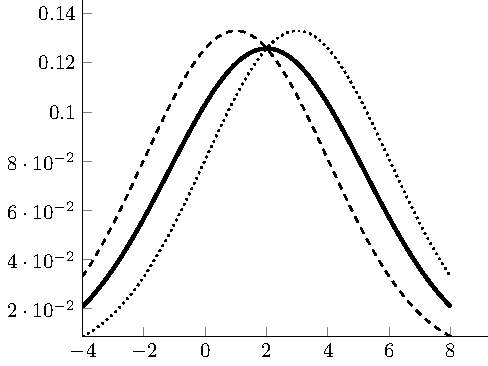
\includegraphics{figures/shortcomings-a.pdf}
    }

    (a)
  \end{minipage}\begin{minipage}{0.5\textwidth}
    \centering
    \scalebox{1.1}{
      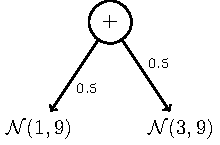
\includegraphics{figures/shortcomings-b.pdf}
    }

    (b)
  \end{minipage}

  \caption[Univariate GSPN in which Max-Product can not find MAP]{
    \textbf{(a)} Plot of the PDFs of three distributions: $X \sim \mathcal{N}(1, 9)$ (dashed line); $X \sim \mathcal{N}(3, 9)$ (dotted line); $X \sim 0.5 \mathcal{N}(1, 9) + 0.5 \mathcal{N}(3, 9)$ (solid line).
    \textbf{(b)} GSPN representing the distribution plotted as a solid line in (a). The approximation algorithms based on Max-Product, seen in Section \ref{sec:map:approximate}, are unable to find its unique mode, $X = 2$.
  }
  \label{fig:shortcomings}
\end{figure}

A common approach to enhance the approximate solutions obtained by these algorithms in discrete SPNs is to perform a \textbf{local search} in the space of possible assignments \citep{Maua2020}. This method involves iteratively modifying individual variable assignments to improve an existing solution. While this approach is straightforward for variable indicators or categorical random variables, adapting it to continuous SPNs, like GSPNs, could involve employing a hill-climbing method such as Modal EM. To illustrate this, Example \ref{ex:shortcomings} shows the application of Modal EM to the SPNs in Figures \ref{fig:shortcomings} and \ref{fig:gspn}.

\begin{example}
  \label{ex:shortcomings}
  \textbf{(a)} Consider the univariate GSPN shown in Figure \ref{fig:shortcomings}. Suppose an approximation algorithm has found the MAP solution $X = 1$, denoted as $x^{(0)}$. By applying Modal EM iteratively, we can observe its convergence towards the mode of the model, the value $X = 2$:

  \begin{minipage}{0.45\textwidth}
    \begin{eqnarray*}
      x^{(0)} & = & 1 \, ; \\
      x^{(1)} & \gets & 1.88934389 \, ; \\
      x^{(2)} & \gets & 1.98770550 \, ; \\
      x^{(3)} & \gets & 1.99863394 \, ;
    \end{eqnarray*}
  \end{minipage}\begin{minipage}{0.45\textwidth}
    \begin{eqnarray*}
      x^{(4)} & \gets & 1.99984822 \, ; \\
      x^{(5)} & \gets & 1.99998314 \, ; \\
      x^{(6)} & \gets & 1.99999813 \, ; \\
      x^{(7)} & \gets & 1.99999979 \, .
    \end{eqnarray*}
  \end{minipage}

  \vspace{1.5em}

  \noindent \textbf{(b)} Now consider the bivariate GSPN shown in Figure \ref{fig:gspn}. Applying Modal EM starting from the solution found by the Max-Product illustration in Figure \ref{fig:maxproduct}, $\mathbf{X} = (11, -4)$, we get:

  \begin{minipage}{0.45\textwidth}
    \begin{eqnarray*}
      \mathbf{x}^{(0)} & = & (11, -4) \, ; \\
      \mathbf{x}^{(1)} & \gets & (10.6418764, -3.9869965) \, ; \\
      \mathbf{x}^{(2)} & \gets & (10.5730441, -3.9844986) \, ; \\
      \mathbf{x}^{(3)} & \gets & (10.5580160,  -3.9839568) \, ;
    \end{eqnarray*}
  \end{minipage}\begin{minipage}{0.45\textwidth}
    \begin{eqnarray*}
      \mathbf{x}^{(4)} & \gets & (10.5546503, -3.9838357) \, ; \\
      \mathbf{x}^{(5)} & \gets & (10.5538923, -3.9838086) \, ; \\
      \mathbf{x}^{(6)} & \gets & (10.5537214, -3.9838023) \, ; \\
      \mathbf{x}^{(7)} & \gets & (10.5536829, -3.9838009) \, .
    \end{eqnarray*}
  \end{minipage}

  \vspace{1.5em}
\end{example}

Another possible strategy to perform MAP inference in GSPNs is to run Modal EM starting from multiple initial points, aiming to identify the highest mode among several local modes. However, this approach would face challenges due to the large number of modes typically present in a GSPN, as discussed in Chapter \ref{cap:gmm}.

\subsection{Modal clustering}

Clustering techniques play a crucial role in various data analysis domains, finding applications in areas such as pattern recognition, image analysis, and machine learning. Typically, a cluster is considered a high-density region within the sample space that is well separated from other high-density regions.

The majority of clustering methods categorizes points in a dataset by mean of a distance function. Such methods proceed by selecting a partition of the dataset that optimizes a chosen objective function that favors small intra-cluster distance and large inter-cluster distance. For instance, the classical $k$-means algorithm repeatedly identifies $k$ cluster centers and assigns data points to the nearest cluster center, with the aim of minimizing the squared distances from the clusters \citep{MacQueen1967}.

More recently, an increasing number of researchers have emphasized the importance of more explicitly incorporating density modeling into clustering procedures \citep{Carlsson2013}. In this direction, \citet{Chacon2019} conducted a comparative study of two distinct density-based clustering approaches: mixture model clustering and clustering based on high-density regions. In the case of mixture model clustering, clusters are associated with mixture components centered at their centroids, as inferred from the learned mixture model. On the other hand, clustering based on high-density regions associates clusters with the local maxima of the mixture density, focusing on regions of elevated density within the mixture.

Mixture model clustering offers the ability to explore more complex scenarios compared to modal clustering when the true density aligns with the assumed class of mixture densities. However, when mixture modeling is primarily employed to approximate any density within the dense space of mixture densities, as is often the case with SPNs, the association between clusters and mixture components becomes less reliable, and in that sense modal clustering is a promising approach.

While LearnSPN utilizes hierarchical clustering to construct the network's structure, cluster analysis on learned SPNs remains a largely unexplored field. Modal EM allows us to perform clustering via mode identification using GSPNs by ascending from any given point to a mode, which is considered to be the representative (center) of a cluster.
